% Kopfzeile beim Kapitelanfang:
\fancypagestyle{plain}{
%Kopfzeile links bzw. innen
\fancyhead[L]{\calligra\Large Vorlesung Nr. 16}
%Kopfzeile rechts bzw. außen
\fancyhead[R]{\calligra\Large 03.12.2012}
}
%Kopfzeile links bzw. innen
\fancyhead[L]{\calligra\Large Vorlesung Nr. 16}
%Kopfzeile rechts bzw. außen
\fancyhead[R]{\calligra\Large 03.12.2012}
% **************************************************
\wdh
	Eine Folge komplexer Zahlen $(c_n)n\geq 0$ konvergiert gegen $c \in \C$ wenn gilt:\\
	Für jedes $\e > 0$ gibt es ein $N \in \N$ so dass $n \geq N \Rarr |c_n - c| < \e$\\
	Eine Reihe $\ds\sum_{n=0}^{\infty} c_n$ mit $c_n \in \C$ heißt \ul{absolut} konvergent, wenn die reelle Reihe $\ds\sum_{n=0}^{\infty} |c_n|$ konvergiert.\\
	Absolute Konvergenz \Rarr{} Konvergenz
	Nach 7.15:\\
	Seien $\ds\sum_{n\geq0} c_n = c$ und $\ds\sum_{n\geq0} c'_n = c'$ konvergente komplexe Reihen, mindestens eine absolut konvergent. Dann konvergiert hier Cauchy-Produkt $\ds\sum_{n\geq0} d_n$ mit dem Grenzwert $c \cdot c'$\\
	\ul{Erinnerung}\\
	$d_n = \ds\sum_{n\geq0} c_k \cdot c_{n - k}$\\
\bew
	Wörtlich wie bei reellen Reihen. \qed

\uS{Die komplexe Exponentialfunktion}
\sS{Satz}
Für $z\eC$ konvergiert die "Exponentialreihe"
$$\sum_{n=0}^{∞}\frac{z^n}{n!}=1+\frac{z}{1}+\frac{z^2}{2}+\frac{z^3}{6}+…$$absolut (Somit konvergiert sie)
\bew
$$\sum_{n=0}^{∞}\left|\frac{z^n}{n!}\right|=\sum_{n=0}^{∞}\frac{|z^n|}{n!}=exp(|z|)$$
Bekannt: $exp(|z|)$ konvergiert\qed

\sS{Definition komplexe Exponentialfunktion}
Die komplexe Exponentialfunktion ist die Abbildung $\ds exp:\C →\C\quad exp(z)=\sum_{n=0}^{∞}\frac{z^n}{n!}$

\uS{Eigenschaften}
\sS{Satz}
Seien $z,w\eC$
\begin{enumerate}
\item{$exp(0)=1$ (klar)}
\item{$exp(z+w)=exp(z)+exp(w)$}
\item{$exp(z)≠0,\ exp(z)^{-1}=exp(-z)$}
\item{$exp(\ol{z})=\ol{exp(z)}$ (Komplexe Konjugation)}
\item{Für $x\eR$ ist $|exp(ix)|=1$}
  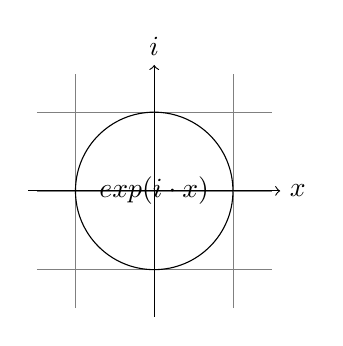
\begin{tikzpicture}[domain=-1.6:1.6,samples=200,prefix=plots/,smooth]
    \draw[very thin,color=gray] (-1.49,-1.49) grid (1.49,1.49);
    \draw[->] (-1.6,0) -- (1.6,0) node[right] {$x$};
    \draw[->] (0,-1.6) -- (0,1.6) node[above] {$i$};
	\draw (0,0) circle (1cm);
	\node (0.5, 0.5) (expo) {$exp(i \cdot x)$};
\end{tikzpicture}
\end{enumerate}
\bew
\begin{enumerate}
\setcounter{enumi}{1}
\item{Wie bei der reellen Exponentialfunktion:\\*
Die Reihe $exp(z+w)$ ist das Cauchy-Produkt der Reihen $exp(z)$ und $exp(w)$, dann folgt $(z)$ aus 7.15}
\item{$exp(z)·exp(-z)\underset{2)}{=}exp(z-z)=exp(0)\underset{1)}{=}1$}
\item{Sei $\ds s_n=\sum_{k=0}^{n}\frac{z^k}{k!}$ somit nach Definition $exp(z)=\lim\limits_{n→∞}s_n$\\*[4pt]
Sei $\ds s_n'=\sum_{k=0}^{n}\frac{\ol{z}^k}{k!}$ somit $exp(\ol{z})=\lim\limits_{n→∞}s_n'$\\*[4pt]
Es gilt $$s_n'=\ol{\sum_{k=0}^{n}\frac{z^k}{k!}}=\sum_{k=0}^{n}\ol{(\frac{z^k}{k!})}=\sum_{k=0}^{n}(\frac{\ol{z}^k}{k!})=s_n'$$
Somit $\ol{exp(z)}=\lim\limits_{\nif}(\ol{s_n})=\lim\limits_{\nif}s_n'=exp(\ol{z})$}
\item{$$|exp(ix)|^2=exp(ix)·\ol{exp(ix)}\underset{4)}{=}exp(ix)·exp(\ol{ix})=exp(ix)·exp(-ix)\underset{2)}{=}exp(ix-ix)=exp(0)\underset{1)}{=}1\ \overset{\sqrt{}}{\Rarr}\ |exp(ix)|=1$$}
\end{enumerate}

\uS{Trigonometrische Funktionen}
\sS{Definition}
Sei $x \in \R$\\*
$sin(x) = Im(exp(i \cdot x))$ (Sinus)\\*
$cos(x) = Re(exp(i \cdot x))$ (Cosinus)\\*
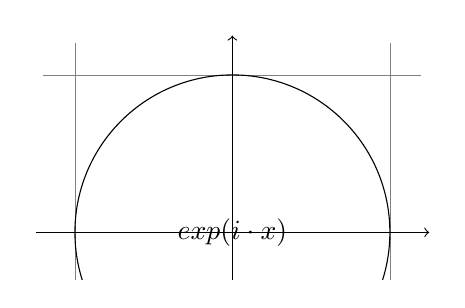
\begin{tikzpicture}[domain=-1.6:1.6, scale=2,samples=200,prefix=plots/,smooth]
	\clip (-1.3,-0.3) rectangle (1.3,1.3);
    \draw[very thin,color=gray] (-1.2,-0.49) grid (1.2,1.2);
    \draw[->] (-1.25,0) -- (1.25,0) node[right] {$x$};
    \draw[->] (0,-1.25) -- (0,1.25) node[above] {$i$};
	\draw (0,0) circle (1);
	\node (0.5, 0.5) (expo) {$exp(i \cdot x)$};
\end{tikzpicture}
\bem
Für jede komplexe Zahl $z$ gilt $z = Re(z) + i \cdot Im(z)$\\*
\Rarr{} $exp(i \cdot x) = cos(x) + i \cdot sin(x)$ (Eulersche Formel)

\sS{Satz}
\begin{enumerate}
\item{$cos(0)=1,\ sin(0)=0$
\begin{tikzpicture}[domain=-4:4,samples=200,prefix=plots/,smooth]
    \draw[very thin,color=gray] (-4,-1.25) grid (4,1.25);
    \draw[->] (-4,0) -- (4,0) node[right] {$x$};
    \draw[->] (0,-1.25) -- (0,1.25) node[above] {$i$};
	\draw[color=red] plot[id=cos] function{cos(x)} node[right] {\footnotesize $f(x) = cos(x)$};
\end{tikzpicture}
}
\item{$cos(-x)=cos(x),\ sin(-x)=-sin(x)$}
\item{$sin(x)^2+cos(x)^2=1$
  \begin{tikzpicture}[domain=-4:4,samples=200,prefix=plots/,smooth]
    \draw[very thin,color=gray] (-4,-1.25) grid (4,1.25);
    \draw[->] (-4,0) -- (4,0) node[right] {$x$};
    \draw[->] (0,-1.25) -- (0,1.25) node[above] {$i$};
	\draw[color=red] plot[id=sin] function{sin(x)} node[right] {\footnotesize $f_1(x) =sin(x)$};
\end{tikzpicture}
}
\item{\desc{Additionstheoreme}{$sin(x+y)=sin(x)·cos(y)+cos(x)·sin(y)$\\*$cos(x+y)=cos(x)·cos(y)-sin(x)·sin(y)$}}
\end{enumerate}
\bew
\begin{enumerate}
\item{$exp(0i)=1=1+0i\ \Rarr\ cos(0)=1, sin(0)=0$}
\item{$exp(-ix)=exp(\ol{ix})=\ol{exp(ix)}=cos(x)-i·sin(x)$\\*
$exp(-ix)=cos(-x)+i·sin{-x}\ \Rarr\ cos(x)=cos(-x),\ sin(-x)=-sin(x)$}
\item{$sin(x)^2+cos(x)^2\overset{Def.}{=}|exp(ix)|^2=1$}
\item{$$exp(i(x+y)) = exp(i \cdot x) \cdot exp(i \cdot y)$$
$$\Rarr cos(x+y) + i \cdot sin(x+y) = (cos(x) + i \cdot sin(x))(cos(y) + i \cdot sin(y))$$
$$=cos(x) \cdot cos(y) - sin(x) \cdot sin(y) + i \cdot (sin(x) \cdot cos(y) + cos(x) \cdot sin(y))$$
Vergleich der Realteile / Imaginärteile \Rarr{} Behauptung 4\qed}
\end{enumerate}
\bem
	Die Gleichung $$cos(x)^2 + sin(x)^2 = 1$$
	impliziert $0 \leq cos(x)^2 \leq 1$, $0 \leq sin(x)^2 \leq 1$ somit $-1 \leq cos(x) \leq 1$, $-1 \leq sin(x) \leq 1$.

\sS{Definition}
	\begin{enumerate}
	\item{Eine Abbildung $f: \C→\C$ heißt stetig in $z \in \C$ wenn gilt:\\*
	Für jedes $\e > 0$ gibt es ein $\delta > 0$ so dass für jedes $w \in \C$ mit $|z - w| < \delta$ ist $|f(z) - f(w)| < \e$}
	\item{$f: \C \to \C$ heißt \ul{stetig}, wenn $f$ in jedem $z \in \C$ stetig ist.}
	\end{enumerate}

\sS{Satz}
Eine Abbildung $f:\C→\C$ ist stetig in $z\eC$ \equ\ Für jede Folge komplexer Zahlen $(z_n)_{n\geq 0}$ mit $z_n→z$ für \nif\ gilt auch $f(z_n)→f(z)$ für \nif
\bew
Wörtlich wie bei reeller Funktion (Satz 6.4)\qed

\sS{Satz}
Die komplexe Exponentialfunktion $exp:\C→\C$ ist stetig
\bew
Verwende Folgenstetigkeit
\begin{enumerate}
\item{Stetigkeit in $z=0\ exp (0)=1$\\*
Sie $z\eC$ (nahe 0)
$$\left|exp(z)-1\right|=\left|1+z+\frac{z^2}{2}+\frac{z^3}{6}+…-1\right|=\left|\sum_{n=1}^{∞}\frac{z^n}{n!}\right|\underset{unendliche Dreiecksungleichung 7.13}{\leq}exp(|z|)-1$$
Wenn $z_n→0$ in \C\\*
dann $|z_n|→0$ in \R\\*
dann $exp(|z_n|) \to exp(0) = 1$ (weil $exp: \R \to \R$ steig)\\*
d.h. $exp(|z_n|) -1 \to 0$\\*
$\Rarr|exp(z_n) - 1| \to 0$\\
Somit $exp$ stetig in $z = 0$ }
\item{Sei $z\eC$ beliebig, $z_n→z$
$$exp(z_n)-exp(z)=exp(z_n-z+z)-exp(z)=exp(z_n-z)-exp(z)-1·exp(z)=(exp(z_n-z)-1)·exp(z)$$
Es gilt: $z_n→z\ \equ\ z_n-z→0$\\*
\alg{&\underset{1)}{\Rarr}\ exp(z_n-z)→1\\
&\equ\ exp(z_n-z)-1→0\\
&\Rarr\ (exp(z_n-z)-1)·exp(z)→0·exp(z)=0
&\underset{(*))}{\Rarr}\ (exp(z_n)-exp(z)→0}
d.h. $exp(z_n)→exp(z)$\qed}
\end{enumerate}

\sS{Satz}
	Die Funktionen $sin: \R \to \R$ und $cos: \R \to \R$ sind stetig.\\
\bew
Mittels Folgenstetigkeit.\\
Sei $x_n \to x$ mit $x_n \in \R,\ x \in \R$\\*
$\Rarr i \cdot x_n \to i \cdot x$ in $\C$\\*
$\underset{7.23}{\Rarr} exp(i \cdot x_n) \to exp(i \cdot x)$\\*
d.h. $cos(x_n) + i \cdot sin(x_n) \to cos(x_n) + i \cdot sin(x_n)$\\*
$\equ cos(x_n) \to cos(x)$ und $sin(x_n) \to sin(x)$\\*
Somit sind $sin$ und $cos$ stetig in $x$ also stetig.